\documentclass[a4paper]{scrartcl}
\usepackage[utf8]{inputenc}
\usepackage[english]{babel}
\usepackage{graphicx}
\usepackage{lastpage}
\usepackage{pgf}
\usepackage{wrapfig}
\usepackage{fancyvrb}
\usepackage{fancyhdr}
\pagestyle{fancy}

\usepackage[backend=bibtex, citestyle=numeric-comp, bibstyle=ieee]{biblatex}
%\addbibresource{ref.bib} % The file containing our references, in BibTeX format
\usepackage{hyperref}
\usepackage{listings}
\usepackage{subcaption}
\usepackage{enumitem}
\usepackage[section]{placeins}

% Create header and footer
\headheight 27pt
\pagestyle{fancyplain}
\lhead{\footnotesize{Internet Applications, ID1354}}
\chead{\footnotesize{Tasty Recipes with PHP}}
\rhead{}
\lfoot{}
\cfoot{\thepage\ (\pageref{LastPage})}
\rfoot{}

% Create title page
\title{Tasty Recipes with PHP}
\subtitle{Internet Applications, ID1354}
\author{Julius Recep Colliander Celik - jcelik@kth.se}
\date{\today}

\begin{document}

\maketitle

\section{Introduction}

This assignment was a continuation of the last one, and PHP was used to create a login system, and implement a persistent comment system. PHP was also used for templating and automatic code generation. Two pages were added, some pages were consolidated into one, and some web page components were divided into multiple files. To view the website it is publicly available on the link \href{https://github.com/juliuscc/kth-id1354/tree/master/homework-2}{https://github.com/juliuscc/kth-id1354/tree/master/homework-2}. 

\section{Literature Study}

I used the lecture slides as primary reference, as well as knowing PHP from before.

\section{Method}

I reused the code from the first assignment and modified it to achieve the tasks in this lab. I used VS Code as my text editor and used MAMP as a PHP web server and Database.

\section{Result}

The work done can be divided into four major parts. The first part is using PHP to improve the development experience (chapter \ref{result:php}). Another use of PHP was using PHP to parse an XML file with data (chapter \ref{result:xml}), removing the model from the view. Also an authentication system was created (chapter \ref{result:auth}), as well as a comment management system (chapter \ref{result:comments}).

\subsection{Using PHP to enforce consistency}
\label{result:php}
Both the \texttt{$<$head$>$} part and the navbar was close to identical in every file. Therefore the code was extracted into seperate php-files that could be shared by all view files. As both the \texttt{$<$head$>$} part and the navbar had small changes that were necessary to be different between all pages, they were implemented as functions, which could be called with parameters. As an example the \texttt{write\_header()} function takes one parameter which is the title string. All pages have a different title like \texttt{"Food Calendar | Receps Recept"} or \texttt{"Meatballs - Recipes | Receps Recept"}.

\subsection{Using XML to store recipe data}
\label{result:xml}
No recipe data is represented anywhere outside the XML file \texttt{cookbook.xml}. It follows the given XML Schema standard. SimpleXML was used to parse the XML-file. Figure \ref{fig:simplexml-code} shows both how SimpleXML was used to parse the xml-file and then how the data structure was used to render recipe-information.

\begin{figure}
\begin{lstlisting}[frame=single, breaklines=true, basicstyle=\ttfamily\footnotesize]
$cookbook = simplexml_load_file("resources/cookbook.xml");
$recipe = $cookbook->recipe[$recipe_index];
.
.
.
<div class="recipe-information">
	<span class="recipe-information__item recipe-information__item--right-divider"><?php echo $recipe->totaltime ?></span>
	<span class="recipe-information__item"><?php echo $recipe->rating ?></span>
	<span class="recipe-information__item recipe-information__item--float--right"><?php echo $recipe->quantity ?></span>
	<p class="recipe-information__description"><?php echo $recipe->description ?></p>
</div>
\end{lstlisting}
\caption{Parts of recipe\_page.php that show the recipe-xml file being used using SimpleXML}
\label{fig:simplexml-code}
\end{figure}



\subsection{Authentication}
\label{result:auth}
A login button was added to the navbar, and it redirects the user to a login page. From the login page, the user can also choose to register a new user which redirects the user to a register page. The login page looked like in figure \ref{fig:login-page}. When a user logs in they are redirected to the home page and they are logged in. They can now write comments and delete their own comments.

\begin{figure}
	\begin{center}
		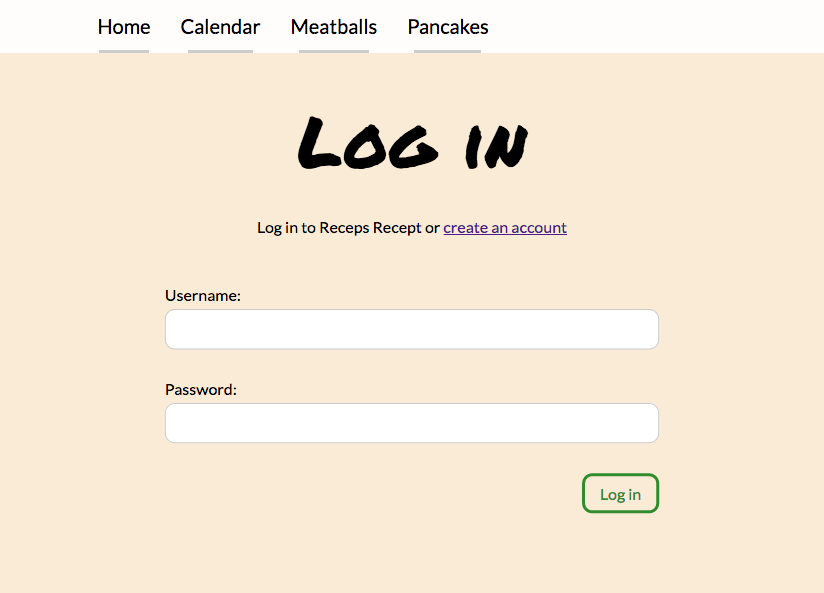
\includegraphics[width=0.7\linewidth]{images/screenshot-login_page.png}
		\caption{Screenshot of the login page}
		\label{fig:login-page}
	\end{center}
\end{figure}

The login page used a form. When that form was submitted it triggered a post to the same page. The PHP code checks if a user exists in a MySQL database, with the given username and password. If the login is successful a session is started and a session variable is initiated. All the other pages uses this session parameter to check if the user is logged in, and the users username. The relevant code is shown in figure \ref{fig:login-code}.

\begin{figure}
\begin{lstlisting}[frame=single, numbers=left, breaklines=true, basicstyle=\ttfamily\footnotesize, firstnumber=13]
if ($_SERVER["REQUEST_METHOD"] == "POST") {
  $username = $_POST['username'];
  $password = $_POST['password'];
  $query = "SELECT * FROM users WHERE username = '$username' and password = '$password'";
	
  $result = mysqli_query($db, $query) or die('Oops something broke! Please try again at a later time.');
  $row = mysqli_fetch_array($result, MYSQLI_ASSOC);
  
  $count = mysqli_num_rows($result);
  if ($count == 1) {
    $_SESSION['active_user'] = $username;
    header("location: index.php");
  } else {
    $error = true;
  }
}
\end{lstlisting}
\caption{Part of login.php that handles log in}
\label{fig:login-code}
\end{figure}

\subsection{Comment management}
\label{result:comments}
When a user is logged in they can se the input form for writing new comments and also the buttons for deleting comments. Figure \ref{fig:comment-section} shows a screenshot of the interface. To create a consistent design even the comments that the user can not delete have a delete button next to them, however the \texttt{visibility} is set to \texttt{hidden}, as shown in figure \ref{fig:comment-section-code}.

\begin{figure}
	\begin{center}
		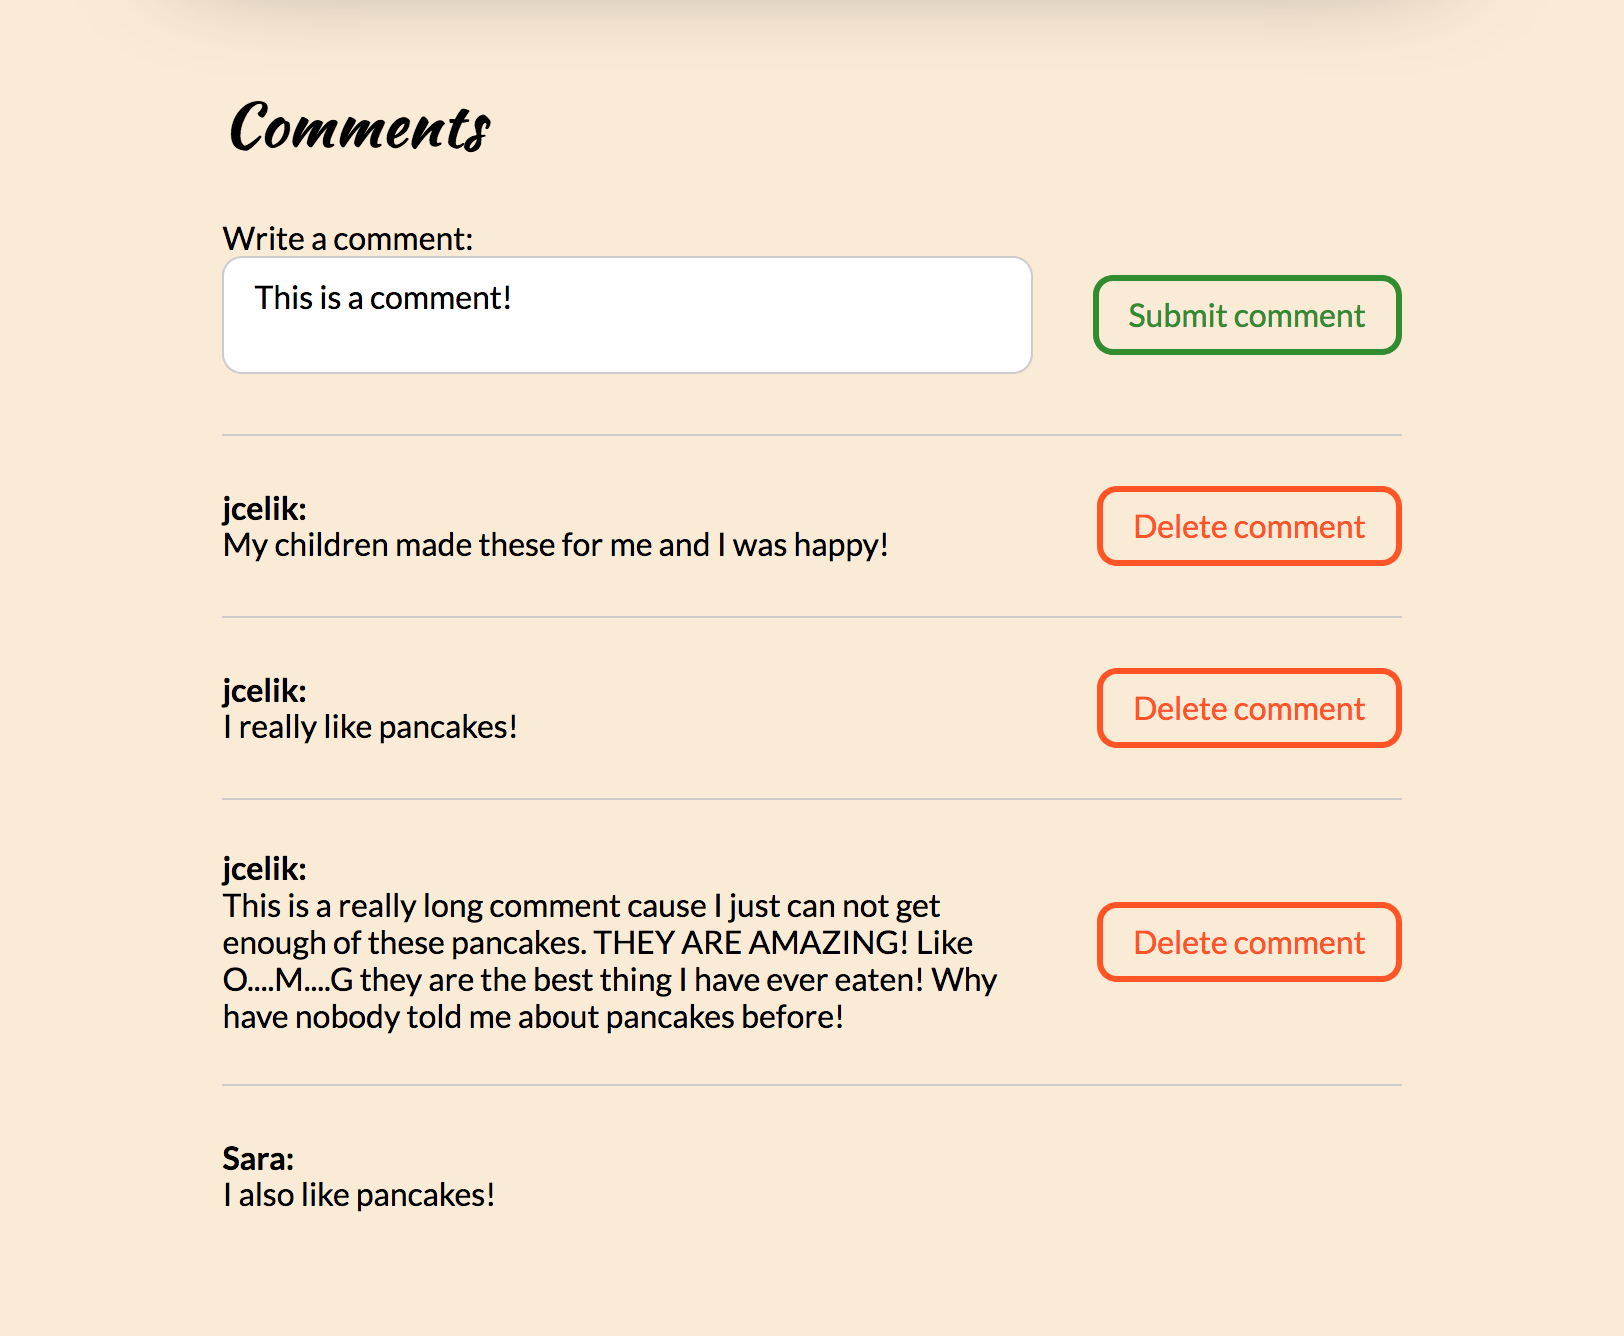
\includegraphics[width=0.7\linewidth]{images/screenshot-comment.png}
		\caption{Screenshot of the comment section of a recipe}
		\label{fig:comment-section}
	\end{center}
\end{figure}

\begin{figure}
\begin{lstlisting}[frame=single, numbers=left, breaklines=true, basicstyle=\ttfamily\footnotesize, firstnumber=101]
if ($current_user === $row["username"]) {
  echo '<button type="submit" class="button button--danger">Delete comment</button>';
} else {
  echo '<button type="submit" style="visibility:hidden" class="button button--danger">Delete comment</button>';
}
\end{lstlisting}
\caption{Part of recipe\_page.php that handles delete buttons rendering}
\label{fig:comment-section-code}
\end{figure}

When a user presses the button they post form data with invisible input fields to \texttt{delete\_user\_comment.php}. One of the hidden input fields is the recipe index so that the user is redirected back to the same recipe page. The code for deleting a comment and submitting a new comment is very similar. Figure \ref{fig:comment-delete-code} shows the complete code for deleting a comment.

\begin{figure}
\begin{lstlisting}[frame=single, numbers=left, breaklines=true, basicstyle=\ttfamily\footnotesize]
<?php
include("config.php");
session_start();

$current_user = $_SESSION["active_user"];
$comment_id = intval($_POST['id']);
$recipe_index = intval($_POST['recipe_index']);

$query = "DELETE FROM comments WHERE id = '$comment_id' AND username = '$current_user'";

mysqli_query($db, $query) or die('Oops something broke! Please try again at a later time.');

header("location: recipe_page.php?recipe_index=$recipe_index");
\end{lstlisting}
	\caption{Copy of delete\_user\_comment.php}
	\label{fig:comment-delete-code}
\end{figure}

\section{Discussion}
There were three mandatory and two optional tasks for this assignment. They were:

\begin{enumerate}
\item \textbf{Mandatory:} Authentication
\item \textbf{Mandatory:} Write Comments to Recipes
\item \textbf{Mandatory:} Delete Comments to Recipes
\item \textbf{Optional:} Register New Users
\item \textbf{Optional:} XML
\end{enumerate}

\noindent
Every requirement was met. I have never used sessions in PHP before and it was not that difficult as I thought. As authentication is close to never a good idea to create yourself, I have always used existing authentication solutions before like Passport for express-based web applications written in Node.js. The code I wrote was not incredibly clearly structured or consistent, which is something that I hope will be fixed by using a proper web framework. The distinction between model, view, and controller was very blurry. I could of course have decoupled those myself but that would have created very much more code and would have taken more time. By using a framework all boilerplate is finished so there is no real cost with decoupling. At least if the framework is good.

\section{Comments About the Course}

Nothing has changed since last week so I include the same text for comments about the course:

\textit{I really like that feedback is collected often during the course. It makes me as a student feel appreciated, and it makes me more invested in the course. I like the assignemnts and the lectures. The course website is very clear and structured, as the rest of the course also is. It really helps us when everything is clear from the beginning. The only thing I could complain about now is that all assignments are not available yet. As the slides are available one could study in advance and it could be possible to want to start with the assignments early.}

It took me little more than halve a day to create the website, and about halve a day to write the report.

\end{document}
